\subsection{Algunas nociones de estadística}
Para analizar una serie de datos numéricos nos interesa utilizar herramientas de probabilidad y estadística.
Existen medidas de tendencia central, para establecer un valor que es considerado el ``centro'' de los datos y medidas de dispersión para cuantificar cuán dispersos están los datos respecto a esas medidas de tendencia central. Cuando se realizan pocas mediciones ($n$, número de mediciones chico) hablamos de una \textbf{muestra} y cuando realizamos muchas mediciones ($n\xrightarrow{}\infty$) hablamos de una \textbf{población}.
Para una muestra la medida de tendencia central es el \textbf{promedio} o media aritmética de la muestra
\begin{equation}
    \bar{x} = \sum_{i=1}^n f_i\,x_i
\end{equation}
donde $f_i$ es la frecuencia relativa (fracción de veces que ocurre un evento u observación) y $x_i$ es el valor de cada observación. Las medidas de dispersión son la \textbf{desviación estándar experimental} o desviación estándar de la muestra
\begin{equation}
    S = \sqrt{\frac{\sum_{i=1}^n {(x_i - \bar{x})}^2}{(n - 1)}}
\end{equation}
que es la raíz cuadrada de la \textbf{varianza}, y a partir de la cual se calcula la \textbf{desviación estándar experimental del promedio}
\begin{equation}
    s(\bar{x}) = \frac{S}{\sqrt{n}}
\end{equation}
En el caso de una población ocurre que la medida de tendencia central es la \textbf{media teórica} o \textbf{esperanza de la distribución} $\mu$, y la medida de dispersión es la \textbf{desviación estándar de la distribución} de probabilidad:
\begin{equation} 
\begin{split}
    \mu = \sum_{i=1}^N p_i\,x_i
\end{split},
\quad \quad
\begin{split}
    \sigma = \sqrt{\dfrac{\sum_{i=1}^n {(x_i - \mu)}^2}{N}}
\end{split},
\quad
\begin{split}
    N\gg n
\end{split}
\end{equation} donde $p_i$ tal que $f_i\xrightarrow{n\xrightarrow{}\infty}p_i$ es la probabilidad de cada observación.

\subsubsection{Distribuciones de probabilidad}\label{sec:distribuciones}

Una distribución de probabilidad es una función que asigna a cada valor de una variable aleatoria $x$ la probabilidad de que esa variable tome ese valor. 

La distribución normal o gaussiana es una distribución de probabilidad continua con ancho entre $-\infty$ y $\infty$, simétrica y centrada en $\mu$, dada por la función de densidad de probabilidad:
\begin{equation}
    f(x) = \frac{1}{\sigma\sqrt{2\pi}}\,e^{-\frac{{(x-\mu)}^2}{2\sigma^2}}
\end{equation}
donde $\mu$ es la media y $\sigma$ es la desviación estándar.

\begin{figure}[!htb]
    \centering
    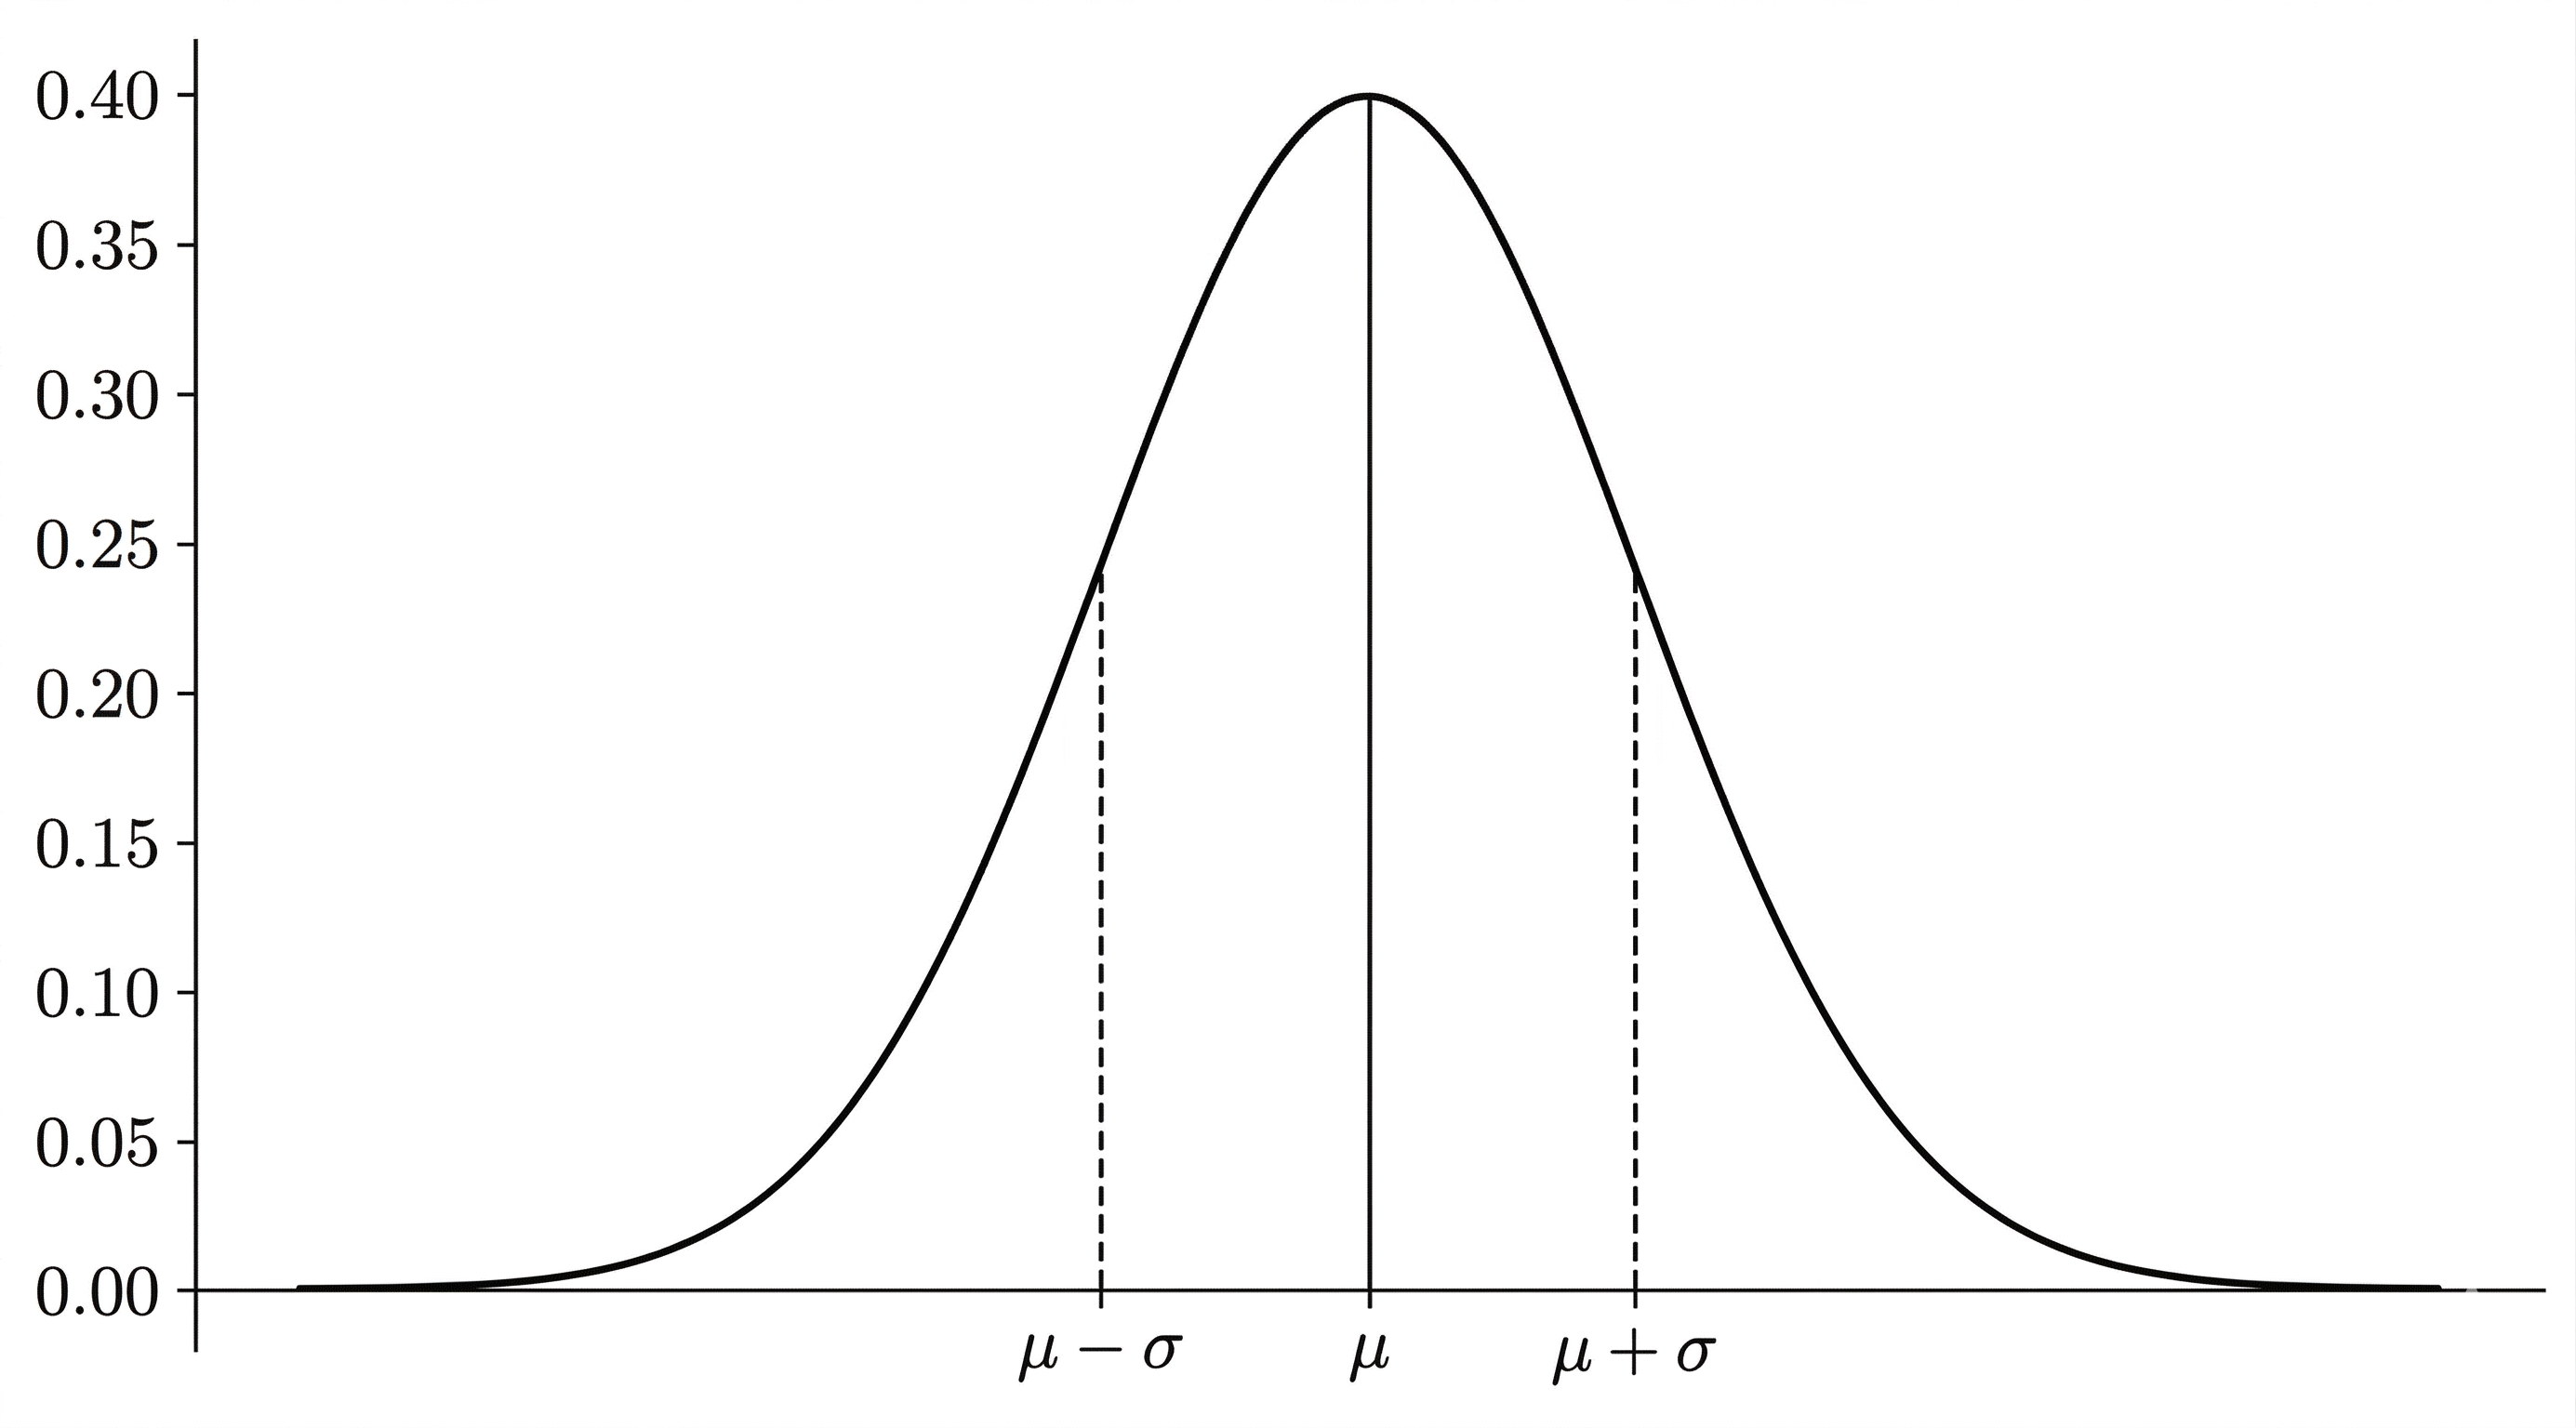
\includegraphics[width=0.6\textwidth]{figures/normal pdf.png}
    \caption{\label{fig:normal_pdf}Normal}
\end{figure}

Cuando tengamos una magnitud de entrada con distribución de origen normal no será necesario ``estandarizar'' la componente de incertidumbre con un factor de estandarización para obtener la incertidumbre típica, porque en ese caso la componente ya viene dada como la desviación estándar (o lo que es lo mismo, tenemos factor de estandarización 1).

La distribución uniforme o rectangular es una distribución de probabilidad continua que le asigna igual probabilidad a todos los resultados dentro de un intervalo $[a, b]$. Su función de densidad de probabilidad es:
\begin{equation}
    f(x) = \begin{cases}
        \frac{1}{b-a} & \text{si } a \leq x \leq b \\
        0 & \text{en otro caso}
    \end{cases}.
\end{equation}

El ancho de la curva es $\Delta = b-a$, la media es $\mu = \frac{a+b}{2}$ y la desviación estándar es $\sigma = \frac{b-a}{\sqrt{12}} = \frac{b-a}{2\sqrt{3}}$.

\begin{figure}[!htb]
    \centering
    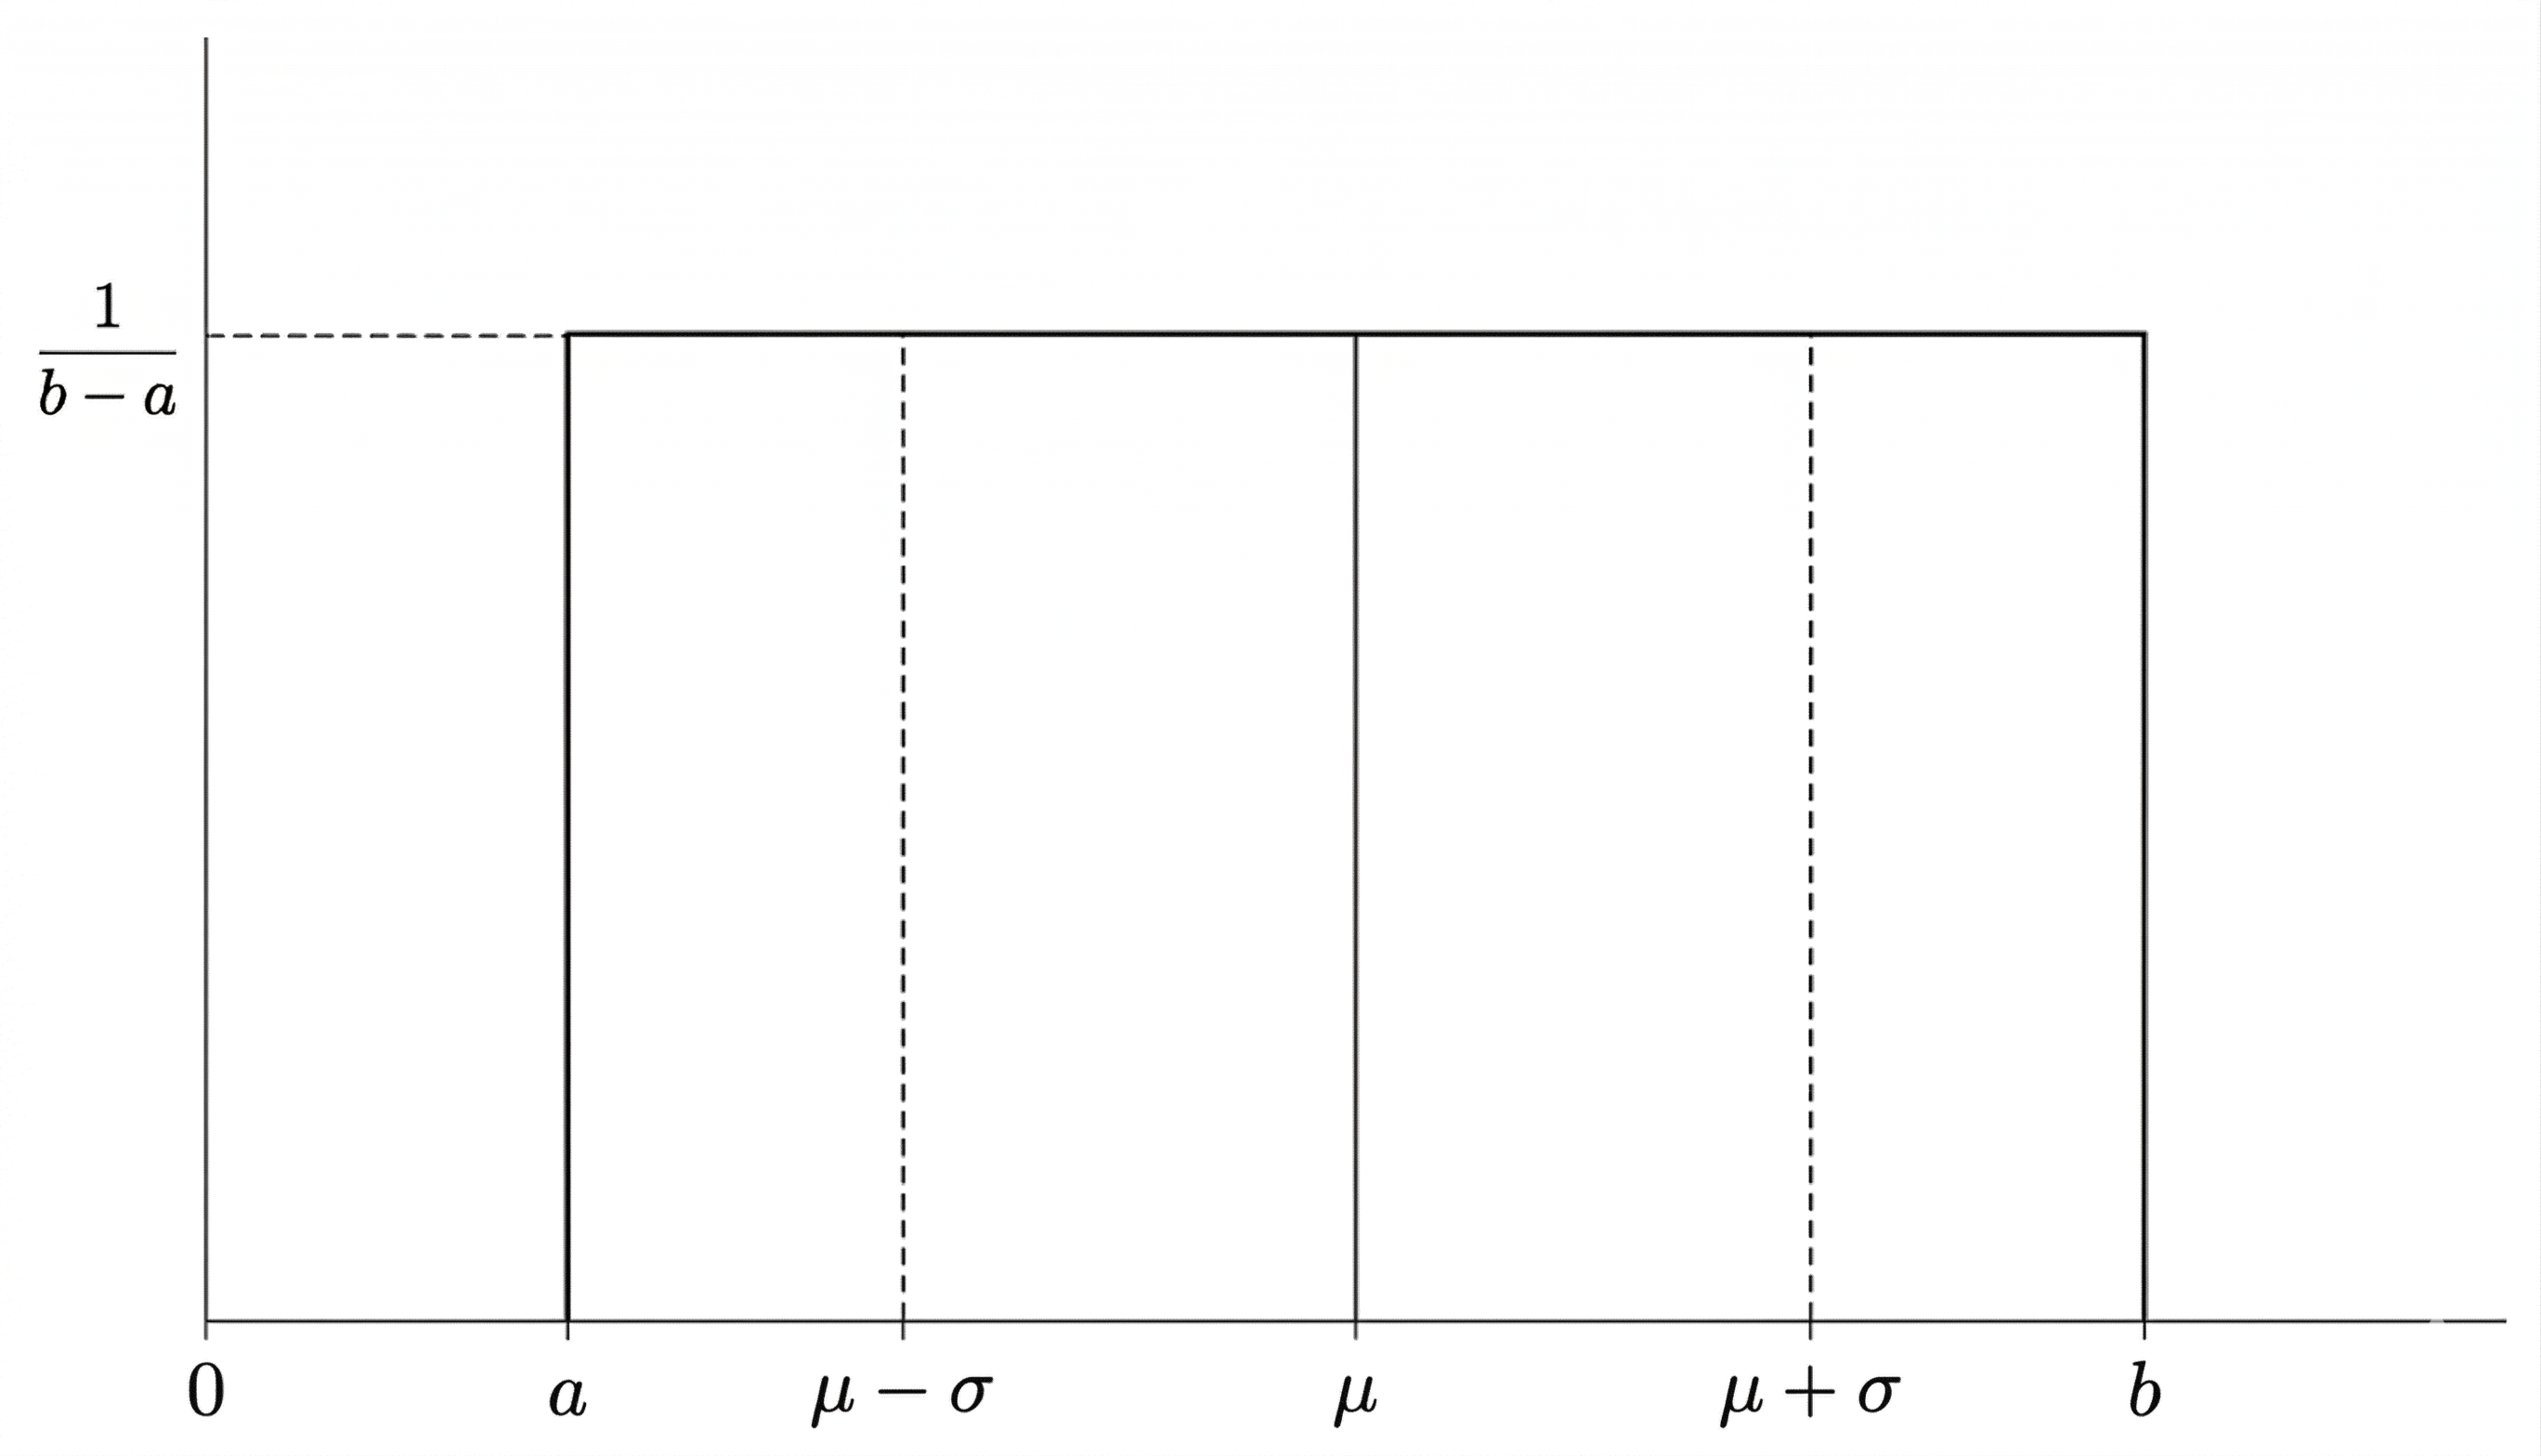
\includegraphics[width=0.6\textwidth]{figures/rectangular pdf.png}
    \caption{\label{fig:rectangular_pdf}Rectangular}
\end{figure}


Cuando tenemos una magnitud de entrada con distribución de origen rectangular, la componente de incertidumbre viene dada como el ancho $\Delta$ o el medio ancho $\frac{\Delta}{2}$ de la curva, y el factor de estandarización necesario para obtener la incertidumbre típica será $\frac{1}{\sqrt{12}}$ o $\frac{1}{\sqrt{3}}$ respectivamente.

La distribución triangular se usa cuando hay poca información disponible sobre la magnitud de entrada, y se conoce o interesa sólo el mínimo, el máximo y el valor más probable.

\begin{figure}[!htb]
    \centering
    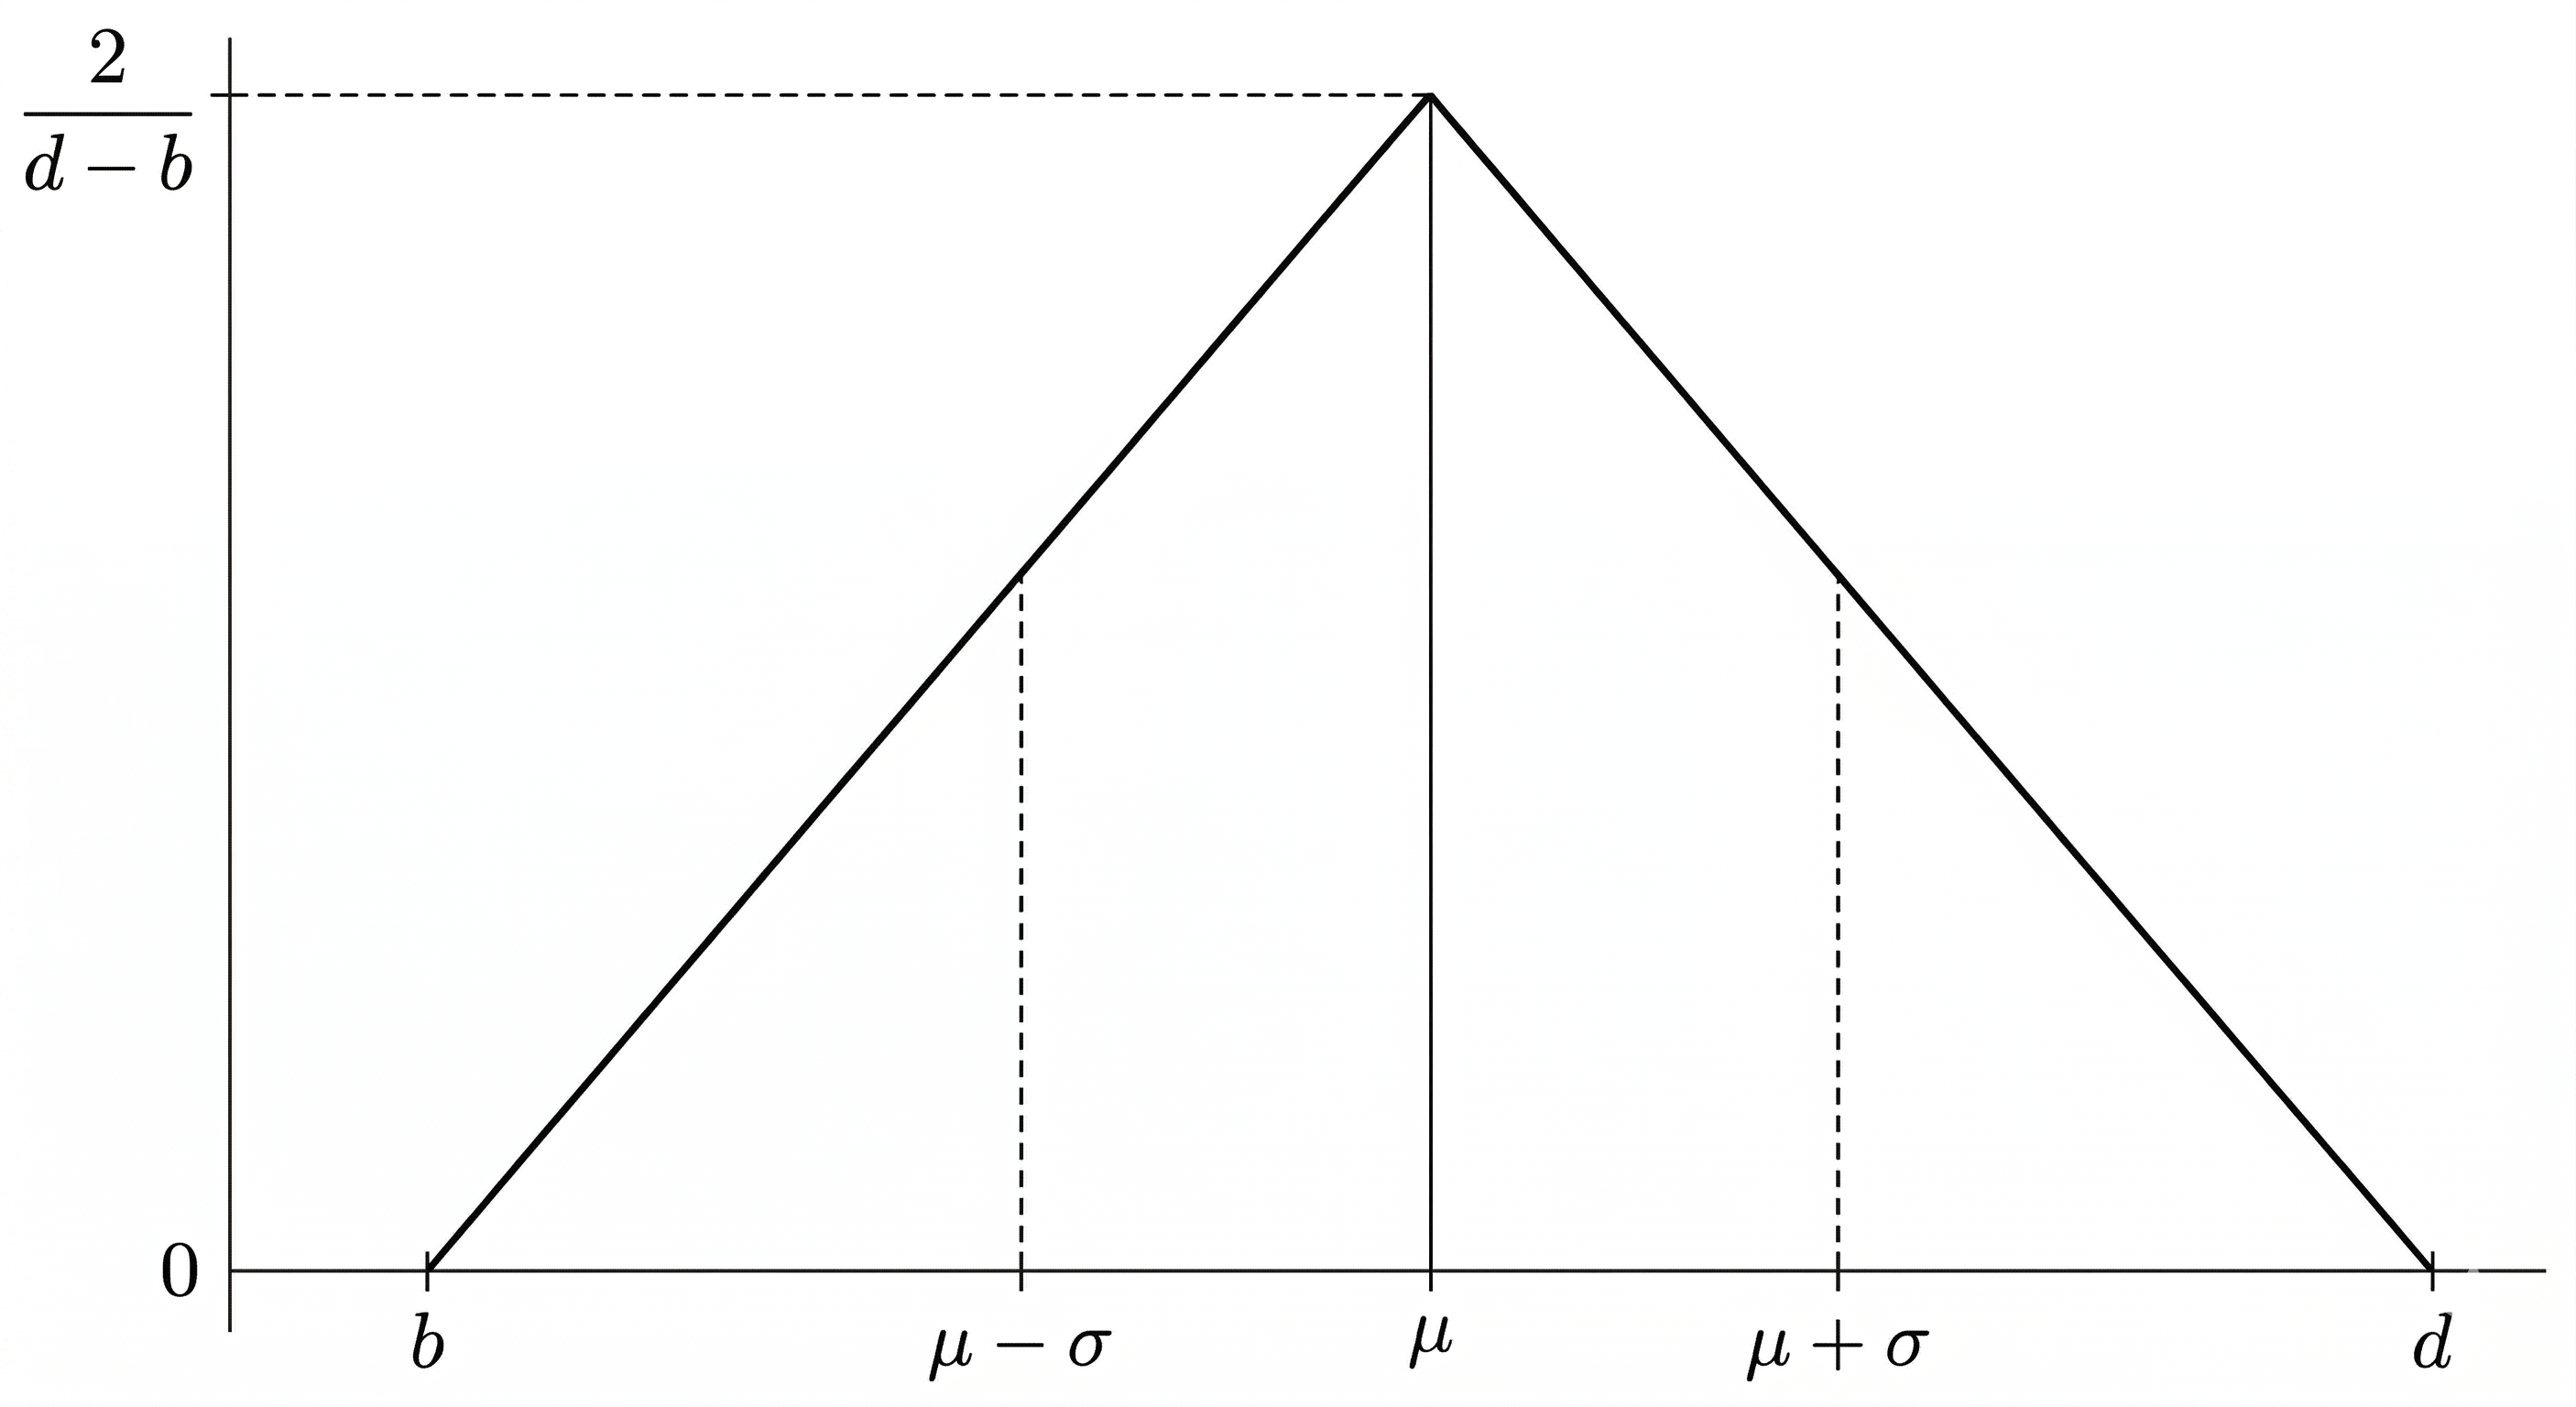
\includegraphics[width=0.6\textwidth]{figures/triangular pdf.png}
    \caption{\label{fig:triangular_pdf}Triangular}
\end{figure}

Cuando es simétrica respecto a la esperanza $\mu = \frac{b+d}{2}$, el ancho de la curva es $\Delta = d-b$ y la desviación estándar es $\sigma = \frac{d-b}{2\sqrt{6}}$. La componente de incertidumbre viene dada como el ancho $\Delta$ o el medio ancho $\frac{\Delta}{2}$ de la curva, y el factor de estandarización necesario para obtener la incertidumbre típica será $\frac{1}{2\sqrt{6}}$ o $\frac{1}{\sqrt{6}}$ respectivamente.